\documentclass{article}

\usepackage[scale=.85]{geometry}
\usepackage[raster]{tcolorbox}
\usepackage{lphandout}

\setmainfont{Fira Sans}
\setmathfont{Fira Math}

\newtcolorbox{ladderbox}[1][]{%
  detach title,
  coltitle=black,
  colback=white,
  before upper={\makebox[3em]{\textbf{Q\thetcbrasternum.}}},
  #1}

\usetikzlibrary{
  matrix,
  matrix.skeleton,
  arrows.meta
}

\ExplSyntaxOn
\tl_new:N \l__ladder_tl
\int_new:N \l__ladder_int
\cs_new_protected:Nn \asxutils_tl_put_right_braced:Nn
 {
  \tl_put_right:Nn #1 { { #2 } }
 }
\cs_new_protected:Nn \asxutils_tl_set_braced:Nn
 {
  \tl_set:Nn #1 { { #2 } }
 }
\cs_new_protected:Nn \asxutils_tl_brace:N
 {
   \asxutils_tl_set_braced:NV #1#1
 }
\cs_generate_variant:Nn \asxutils_tl_put_right_braced:Nn { NV, cV, cv, Nx, cx }
\cs_generate_variant:Nn \asxutils_tl_set_braced:Nn { NV, cV, cv, Nx, cx }

\cs_new_protected_nopar:Npn \make_ladder:n #1
{
  \tl_clear:N \l__ladder_tl
  \int_set:Nn \l__ladder_int {\clist_count:n {#1}}
  \clist_map_inline:nn {#1}{
    \tl_put_right:Nn \l__ladder_tl
    {
      ##1 \& \\
    }
  }
  \asxutils_tl_brace:N \l__ladder_tl
  
  \tl_put_left:Nn \l__ladder_tl
  {
    \matrix[
      matrix~ of~ nodes,
      nodes~ in~ empty~ cells,
      label~ skeleton,
      ampersand~ replacement=\&,
      column~ 1/.style={
        minimum~height=1.5em,
        minimum~width=6ex,
      }
    ] (-ladder)
  }
  \tl_put_right:Nn \l__ladder_tl {;}
  \tl_use:N \l__ladder_tl

  \draw[ultra~ thick] (-ladder-column-1.north~ east) -- (-ladder-column-1.south~ east);
  \draw[ultra~ thick] (-ladder-column-1.north~ west) -- (-ladder-column-1.south~ west);
  \foreach \k in {2,...,\int_use:N \l__ladder_int} {
    \draw[ultra~ thick] (-ladder-cell-\k-1.north~ east) --  (-ladder-cell-\k-1.north~ west);
  }
}


\tikzset{
  ladder/.pic={
    \make_ladder:n {#1}
  }
}
\ExplSyntaxOff

\NewDocumentCommand \Ladder {m}
{%
  \begin{ladderbox}
\begin{tikzpicture}[>=Latex,baseline={(0,0)}]
\pic {ladder={#1}};
\end{tikzpicture}
  \end{ladderbox}%
}%

\title{Word Ladders}
\author{ASX}

\begin{document}

\begin{center}
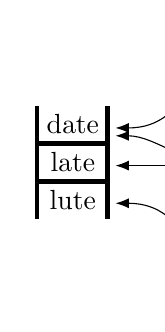
\begin{tikzpicture}[>=Latex]
\matrix[
  matrix of nodes,
  nodes in empty cells,
  label skeleton,
] (ladder) {
  date& \\
  late& \\
  lute& \\
};
\begin{scope}[
  local bounding box=annotations
]
\draw[ultra thick] (ladder-column-1.north east) -- (ladder-column-1.south east);
\draw[ultra thick] (ladder-column-1.north west) -- (ladder-column-1.south west);
\foreach \k in {1,2} {
  \draw[ultra thick] (ladder-cell-\k-1.south east) --  (ladder-cell-\k-1.south west);
}
\draw[<-] (ladder-1-1.mid east -| ladder-column-1.east) +(.1,0) .. controls +(1,0) and +(-1,0) .. +(2,1) node[right] {Starting word};
\draw[<-] (ladder-3-1.mid east -| ladder-column-1.east) +(.1,0) .. controls +(1,0) and +(-1,0) .. +(2,-1) node[right] {Target word};
\draw[<-] (ladder-2-1.mid east -| ladder-column-1.east) +(.1,0) -- +(1.5,0) coordinate (a) -- +(2,0) node[right] {Differ by one letter};

\draw[<-] (ladder-1-1.mid east -| ladder-column-1.east) +(.1,-.1) .. controls +(.5,0) and +(-.5,0) .. (a);
\end{scope}
\pgfresetboundingbox
\path[use as bounding box]
(ladder.east |- annotations.south) rectangle (ladder.west |- annotations.north);
\end{tikzpicture}
\end{center}

\begin{tcbraster}[
  raster columns=4,
  raster equal height=rows,
]
\Ladder{earn,{},burn} % pattern 0,1
\Ladder{boar,{},near} % pattern 0,1
\Ladder{wise,{},rice} % pattern 0,2
\Ladder{boil,{},bait} % pattern 1,3
\Ladder{east,{},{},poet} % pattern 0,1,2
\Ladder{shop,{},{},stem} % pattern 1,2,3
\Ladder{bake,{},{},lime} % pattern 1,0,2
\Ladder{pink,{},{},five} % pattern 3,0,2
\Ladder{ware,{},{},{},film} % pattern 0,1,2,3
\Ladder{land,{},{},{},belt} % pattern 0,1,3,2
\Ladder{bold,{},{},{},seat} % pattern 3,2,1,0
\Ladder{cold,{},{},{},save} % pattern 0,3,1,2
\Ladder{pale,{},{mile},{},{},wind} % pattern 0,1,2,3,0
\Ladder{dale,{},{},{},{},most} % pattern 0,1,2,3,0
\Ladder{none,{},{},{},{},hack} % pattern 0,1,2,3,0
\Ladder{fame,{},{},{},{},gold} % pattern 0,1,2,3,0
\Ladder{bare,{},{cure},{},{},city} % pattern 0,1,2,1,3
\Ladder{that,{},{},{},{},cash} % pattern 0,1,2,1,3
\Ladder{junk,{},{},{},{},pace} % pattern 0,1,2,1,3
\Ladder{site,{},{},{},{},cart} % pattern 0,1,2,1,3
\end{tcbraster}

\end{document}
